% Neural network diagram
% Made with Xematics. Positions are in px (1 px = 0.75 pt), as in the SVG export.
\documentclass[tikz, border=4pt]{standalone}
\definecolor{xm1}{HTML}{FFFFFF}
\definecolor{xm2}{HTML}{F6EFA6}
\definecolor{xm3}{HTML}{8A7F00}
\definecolor{xm4}{HTML}{E69F00}
\definecolor{xm5}{HTML}{D55E00}
\definecolor{xm6}{HTML}{C3C8CF}
\definecolor{xm7}{HTML}{56B4E9}
\definecolor{xm8}{HTML}{0072B2}
\definecolor{xm9}{HTML}{D1D5DB}
\definecolor{xm10}{HTML}{6B7280}
\definecolor{xm11}{HTML}{4B5563}
\definecolor{xm12}{HTML}{B3B8BF}
\definecolor{xm13}{HTML}{1F2937}
\begin{document}
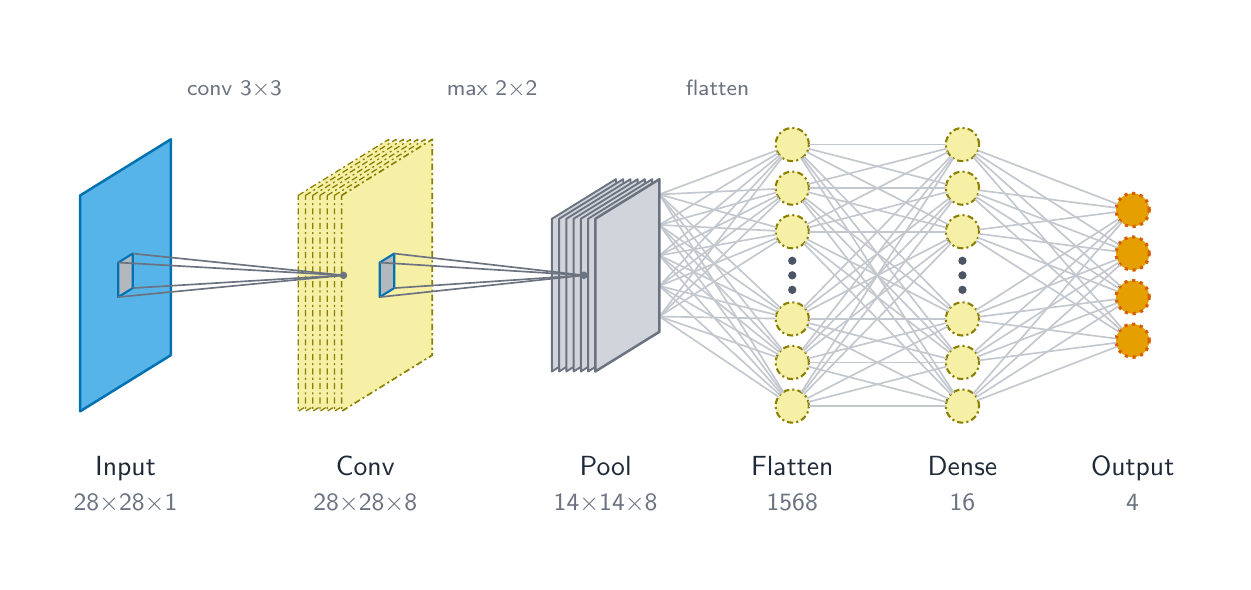
\begin{tikzpicture}[x=0.75pt, y=-0.75pt]
  \tikzset{
    xm hidden/.style={circle, minimum size=12pt, inner sep=0, outer sep=0, fill=xm2, draw=xm3, line width=0.75pt, dash pattern=on 2.25pt off 1.13pt on 0.75pt off 1.13pt},
    xm output/.style={circle, minimum size=12pt, inner sep=0, outer sep=0, fill=xm4, draw=xm5, line width=1.13pt, dash pattern=on 1.13pt off 1.69pt},
    xm edge/.style={draw=xm6, line width=0.6pt},
    xm map input/.style={fill=xm7, draw=xm8, line width=0.9pt, line join=round},
    xm map hidden back/.style={fill=xm2, draw=xm3, line width=0.45pt, dash pattern=on 2.25pt off 1.13pt on 0.75pt off 1.13pt, line join=round},
    xm map hidden/.style={fill=xm2, draw=xm3, line width=0.6pt, dash pattern=on 2.25pt off 1.13pt on 0.75pt off 1.13pt, line join=round},
    xm map pool back/.style={fill=xm9, draw=xm10, line width=0.68pt, line join=round},
    xm map pool/.style={fill=xm9, draw=xm10, line width=0.9pt, line join=round},
    xm dots/.style={fill=xm11},
    xm window/.style={fill=xm12, draw=xm8, line width=0.75pt, line join=round},
    xm ray/.style={draw=xm10, line width=0.6pt},
    xm ray end/.style={fill=xm10},
    xm name xm13/.style={text=xm13, inner sep=0, font=\sffamily\fontsize{9.75}{11.7}\selectfont},
    xm size xm10/.style={text=xm10, inner sep=0, font=\sffamily\fontsize{9}{10.8}\selectfont},
    xm op xm10/.style={text=xm10, inner sep=0, font=\sffamily\fontsize{8.25}{9.9}\selectfont},
  }
  \fill[xm1] (0,0) rectangle (575.62,257.56);
  % Neurons
  \node[xm hidden] (n-3-0) at (368.37,56.31) {};
  \node[xm hidden] (n-3-1) at (368.37,77.31) {};
  \node[xm hidden] (n-3-2) at (368.37,98.31) {};
  \node[xm hidden] (n-3-1565) at (368.37,140.31) {};
  \node[xm hidden] (n-3-1566) at (368.37,161.31) {};
  \node[xm hidden] (n-3-1567) at (368.37,182.31) {};
  \node[xm hidden] (n-4-0) at (450.37,56.31) {};
  \node[xm hidden] (n-4-1) at (450.37,77.31) {};
  \node[xm hidden] (n-4-2) at (450.37,98.31) {};
  \node[xm hidden] (n-4-13) at (450.37,140.31) {};
  \node[xm hidden] (n-4-14) at (450.37,161.31) {};
  \node[xm hidden] (n-4-15) at (450.37,182.31) {};
  \node[xm output] (n-5-0) at (532.37,87.81) {};
  \node[xm output] (n-5-1) at (532.37,108.81) {};
  \node[xm output] (n-5-2) at (532.37,129.81) {};
  \node[xm output] (n-5-3) at (532.37,150.81) {};
  % Connections 2
  \draw[xm edge] (304.37,80.33) -- (n-3-0);
  \draw[xm edge] (304.37,80.33) -- (n-3-1);
  \draw[xm edge] (304.37,80.33) -- (n-3-2);
  \draw[xm edge] (304.37,80.33) -- (n-3-1565);
  \draw[xm edge] (304.37,80.33) -- (n-3-1566);
  \draw[xm edge] (304.37,80.33) -- (n-3-1567);
  \draw[xm edge] (304.37,95.04) -- (n-3-0);
  \draw[xm edge] (304.37,95.04) -- (n-3-1);
  \draw[xm edge] (304.37,95.04) -- (n-3-2);
  \draw[xm edge] (304.37,95.04) -- (n-3-1565);
  \draw[xm edge] (304.37,95.04) -- (n-3-1566);
  \draw[xm edge] (304.37,95.04) -- (n-3-1567);
  \draw[xm edge] (304.37,109.75) -- (n-3-0);
  \draw[xm edge] (304.37,109.75) -- (n-3-1);
  \draw[xm edge] (304.37,109.75) -- (n-3-2);
  \draw[xm edge] (304.37,109.75) -- (n-3-1565);
  \draw[xm edge] (304.37,109.75) -- (n-3-1566);
  \draw[xm edge] (304.37,109.75) -- (n-3-1567);
  \draw[xm edge] (304.37,124.46) -- (n-3-0);
  \draw[xm edge] (304.37,124.46) -- (n-3-1);
  \draw[xm edge] (304.37,124.46) -- (n-3-2);
  \draw[xm edge] (304.37,124.46) -- (n-3-1565);
  \draw[xm edge] (304.37,124.46) -- (n-3-1566);
  \draw[xm edge] (304.37,124.46) -- (n-3-1567);
  \draw[xm edge] (304.37,139.17) -- (n-3-0);
  \draw[xm edge] (304.37,139.17) -- (n-3-1);
  \draw[xm edge] (304.37,139.17) -- (n-3-2);
  \draw[xm edge] (304.37,139.17) -- (n-3-1565);
  \draw[xm edge] (304.37,139.17) -- (n-3-1566);
  \draw[xm edge] (304.37,139.17) -- (n-3-1567);
  % Connections 3
  \draw[xm edge] (n-3-0) -- (n-4-0);
  \draw[xm edge] (n-3-0) -- (n-4-1);
  \draw[xm edge] (n-3-0) -- (n-4-2);
  \draw[xm edge] (n-3-0) -- (n-4-13);
  \draw[xm edge] (n-3-0) -- (n-4-14);
  \draw[xm edge] (n-3-0) -- (n-4-15);
  \draw[xm edge] (n-3-1) -- (n-4-0);
  \draw[xm edge] (n-3-1) -- (n-4-1);
  \draw[xm edge] (n-3-1) -- (n-4-2);
  \draw[xm edge] (n-3-1) -- (n-4-13);
  \draw[xm edge] (n-3-1) -- (n-4-14);
  \draw[xm edge] (n-3-1) -- (n-4-15);
  \draw[xm edge] (n-3-2) -- (n-4-0);
  \draw[xm edge] (n-3-2) -- (n-4-1);
  \draw[xm edge] (n-3-2) -- (n-4-2);
  \draw[xm edge] (n-3-2) -- (n-4-13);
  \draw[xm edge] (n-3-2) -- (n-4-14);
  \draw[xm edge] (n-3-2) -- (n-4-15);
  \draw[xm edge] (n-3-1565) -- (n-4-0);
  \draw[xm edge] (n-3-1565) -- (n-4-1);
  \draw[xm edge] (n-3-1565) -- (n-4-2);
  \draw[xm edge] (n-3-1565) -- (n-4-13);
  \draw[xm edge] (n-3-1565) -- (n-4-14);
  \draw[xm edge] (n-3-1565) -- (n-4-15);
  \draw[xm edge] (n-3-1566) -- (n-4-0);
  \draw[xm edge] (n-3-1566) -- (n-4-1);
  \draw[xm edge] (n-3-1566) -- (n-4-2);
  \draw[xm edge] (n-3-1566) -- (n-4-13);
  \draw[xm edge] (n-3-1566) -- (n-4-14);
  \draw[xm edge] (n-3-1566) -- (n-4-15);
  \draw[xm edge] (n-3-1567) -- (n-4-0);
  \draw[xm edge] (n-3-1567) -- (n-4-1);
  \draw[xm edge] (n-3-1567) -- (n-4-2);
  \draw[xm edge] (n-3-1567) -- (n-4-13);
  \draw[xm edge] (n-3-1567) -- (n-4-14);
  \draw[xm edge] (n-3-1567) -- (n-4-15);
  % Connections 4
  \draw[xm edge] (n-4-0) -- (n-5-0);
  \draw[xm edge] (n-4-0) -- (n-5-1);
  \draw[xm edge] (n-4-0) -- (n-5-2);
  \draw[xm edge] (n-4-0) -- (n-5-3);
  \draw[xm edge] (n-4-1) -- (n-5-0);
  \draw[xm edge] (n-4-1) -- (n-5-1);
  \draw[xm edge] (n-4-1) -- (n-5-2);
  \draw[xm edge] (n-4-1) -- (n-5-3);
  \draw[xm edge] (n-4-2) -- (n-5-0);
  \draw[xm edge] (n-4-2) -- (n-5-1);
  \draw[xm edge] (n-4-2) -- (n-5-2);
  \draw[xm edge] (n-4-2) -- (n-5-3);
  \draw[xm edge] (n-4-13) -- (n-5-0);
  \draw[xm edge] (n-4-13) -- (n-5-1);
  \draw[xm edge] (n-4-13) -- (n-5-2);
  \draw[xm edge] (n-4-13) -- (n-5-3);
  \draw[xm edge] (n-4-14) -- (n-5-0);
  \draw[xm edge] (n-4-14) -- (n-5-1);
  \draw[xm edge] (n-4-14) -- (n-5-2);
  \draw[xm edge] (n-4-14) -- (n-5-3);
  \draw[xm edge] (n-4-15) -- (n-5-0);
  \draw[xm edge] (n-4-15) -- (n-5-1);
  \draw[xm edge] (n-4-15) -- (n-5-2);
  \draw[xm edge] (n-4-15) -- (n-5-3);
  % Layers
  \draw[xm map input] (25.28,80.83) -- (68.96,53.79) -- (68.96,157.79) -- (25.28,184.83) -- cycle;
  \draw[xm map hidden back] (130.32,80.83) -- (174,53.79) -- (174,157.79) -- (130.32,184.83) -- cycle;
  \draw[xm map hidden back] (133.81,80.83) -- (177.49,53.79) -- (177.49,157.79) -- (133.81,184.83) -- cycle;
  \draw[xm map hidden back] (137.3,80.83) -- (180.98,53.79) -- (180.98,157.79) -- (137.3,184.83) -- cycle;
  \draw[xm map hidden back] (140.79,80.83) -- (184.47,53.79) -- (184.47,157.79) -- (140.79,184.83) -- cycle;
  \draw[xm map hidden back] (144.28,80.83) -- (187.96,53.79) -- (187.96,157.79) -- (144.28,184.83) -- cycle;
  \draw[xm map hidden back] (147.77,80.83) -- (191.45,53.79) -- (191.45,157.79) -- (147.77,184.83) -- cycle;
  \draw[xm map hidden] (151.26,80.83) -- (194.94,53.79) -- (194.94,157.79) -- (151.26,184.83) -- cycle;
  \draw[xm map pool back] (252.55,92.1) -- (283.43,72.98) -- (283.43,146.52) -- (252.55,165.64) -- cycle;
  \draw[xm map pool back] (256.04,92.1) -- (286.92,72.98) -- (286.92,146.52) -- (256.04,165.64) -- cycle;
  \draw[xm map pool back] (259.53,92.1) -- (290.41,72.98) -- (290.41,146.52) -- (259.53,165.64) -- cycle;
  \draw[xm map pool back] (263.02,92.1) -- (293.9,72.98) -- (293.9,146.52) -- (263.02,165.64) -- cycle;
  \draw[xm map pool back] (266.51,92.1) -- (297.39,72.98) -- (297.39,146.52) -- (266.51,165.64) -- cycle;
  \draw[xm map pool back] (270,92.1) -- (300.88,72.98) -- (300.88,146.52) -- (270,165.64) -- cycle;
  \draw[xm map pool] (273.49,92.1) -- (304.37,72.98) -- (304.37,146.52) -- (273.49,165.64) -- cycle;
  \fill[xm dots] (368.37,112.31) circle[radius=2];
  \fill[xm dots] (368.37,119.31) circle[radius=2];
  \fill[xm dots] (368.37,126.31) circle[radius=2];
  \fill[xm dots] (450.37,112.31) circle[radius=2];
  \fill[xm dots] (450.37,119.31) circle[radius=2];
  \fill[xm dots] (450.37,126.31) circle[radius=2];
  \draw[xm window] (43.63,113.15) -- (50.62,108.83) -- (50.62,125.47) -- (43.63,129.79) -- cycle;
  \draw[xm ray] (43.63,113.15) -- (152.16,119.31);
  \draw[xm ray] (50.62,108.83) -- (152.16,119.31);
  \draw[xm ray] (50.62,125.47) -- (152.16,119.31);
  \draw[xm ray] (43.63,129.79) -- (152.16,119.31);
  \fill[xm ray end] (152.16,119.31) circle[radius=1.8];
  \draw[xm window] (169.61,113.15) -- (176.6,108.83) -- (176.6,125.47) -- (169.61,129.79) -- cycle;
  \draw[xm ray] (169.61,113.15) -- (267.99,119.31);
  \draw[xm ray] (176.6,108.83) -- (267.99,119.31);
  \draw[xm ray] (176.6,125.47) -- (267.99,119.31);
  \draw[xm ray] (169.61,129.79) -- (267.99,119.31);
  \fill[xm ray end] (267.99,119.31) circle[radius=1.8];
  % Labels
  \node[xm name xm13, anchor=base] at (47.12,215.9) {Input};
  \node[xm size xm10, anchor=base] at (47.12,232.66) {28\ensuremath{\times}28\ensuremath{\times}1};
  \node[xm op xm10, anchor=base] at (99.64,32.66) {conv 3\ensuremath{\times}3};
  \node[xm name xm13, anchor=base] at (162.63,215.9) {Conv};
  \node[xm size xm10, anchor=base] at (162.63,232.66) {28\ensuremath{\times}28\ensuremath{\times}8};
  \node[xm op xm10, anchor=base] at (223.75,32.66) {max 2\ensuremath{\times}2};
  \node[xm name xm13, anchor=base] at (278.46,215.9) {Pool};
  \node[xm size xm10, anchor=base] at (278.46,232.66) {14\ensuremath{\times}14\ensuremath{\times}8};
  \node[xm op xm10, anchor=base] at (332.37,32.66) {flatten};
  \node[xm name xm13, anchor=base] at (368.37,215.9) {Flatten};
  \node[xm size xm10, anchor=base] at (368.37,232.66) {1568};
  \node[xm name xm13, anchor=base] at (450.37,215.9) {Dense};
  \node[xm size xm10, anchor=base] at (450.37,232.66) {16};
  \node[xm name xm13, anchor=base] at (532.37,215.9) {Output};
  \node[xm size xm10, anchor=base] at (532.37,232.66) {4};
\end{tikzpicture}
\end{document}
